\documentclass[12pt,ngerman]{dtk}
\usepackage[utf8]{inputenc}
\usepackage[]{hyperref}
\usepackage[]{babel}
\usepackage[]{csquotes}
\usepackage{blindtext}
\usepackage[]{booktabs}
\usepackage[]{listings}
\usepackage[]{microtype}
\usepackage[]{paralist} 
\usepackage[]{xcolor,xspace}
\usepackage{siunitx}

\sisetup{
output-decimal-marker = {,}}


\Author{Uwe}{Ziegenhagen}{Köln} 
\markboth{Euro\TeX~2012}{Euro\TeX~2012}


\title{Klompen, Kaas \&  Con\TeX t -- Die Euro\TeX~2012 \\ in Breskens}
\begin{document}
\maketitle

\begin{abstract}
Wieder einmal habe ich den Fehler begangen, mich am ersten Abend einer Dante-Tagung in die Nähe des
 DTK Chefredakteurs Herbert  zu begeben. Ich weiß auch nicht, ob es an der guten Stimmung lag oder
 ob das Mineralwasser bewusstseinsverändernde Substanzen enthielt (man war ja schließlich in den
 Niederlanden), auf jeden Fall habe ich zu schnell zugesagt, als es darum ging, den Tagungsbericht zu
 verfassen. Hier nun mein Bericht\dots
\end{abstract}


\section{Anreise}

Die Euro\TeX~2012 fand im niederländischen Breskens statt, in dem Teil des Landes, der nur per Fähre,
 Tunnel oder über Belgien erreichbar ist. Dank der offenen Grenzen ist die freie Fahrt aber kein Problem,
 man merkt kaum, in welchem Land man gerade unterwegs ist.

Die Anreise gestaltete sich für mich als einfach, nachdem Thomas angeboten hatte, mich mit dem Auto
 mitzunehmen. Beladen mit zwei Laptops, diversen iGeräten und umfangreicher Fotoausrüstung ging es
 Sonntagnachmittag los. Dank Navi war die Wegfindung kein Problem, sodass wir kurz nach 20 Uhr im
 Hotel \enquote{Scaldis} empfangen wurden, das für die nächsten Tage unser Zuhause sein sollte.

\begin{figure}
\centering
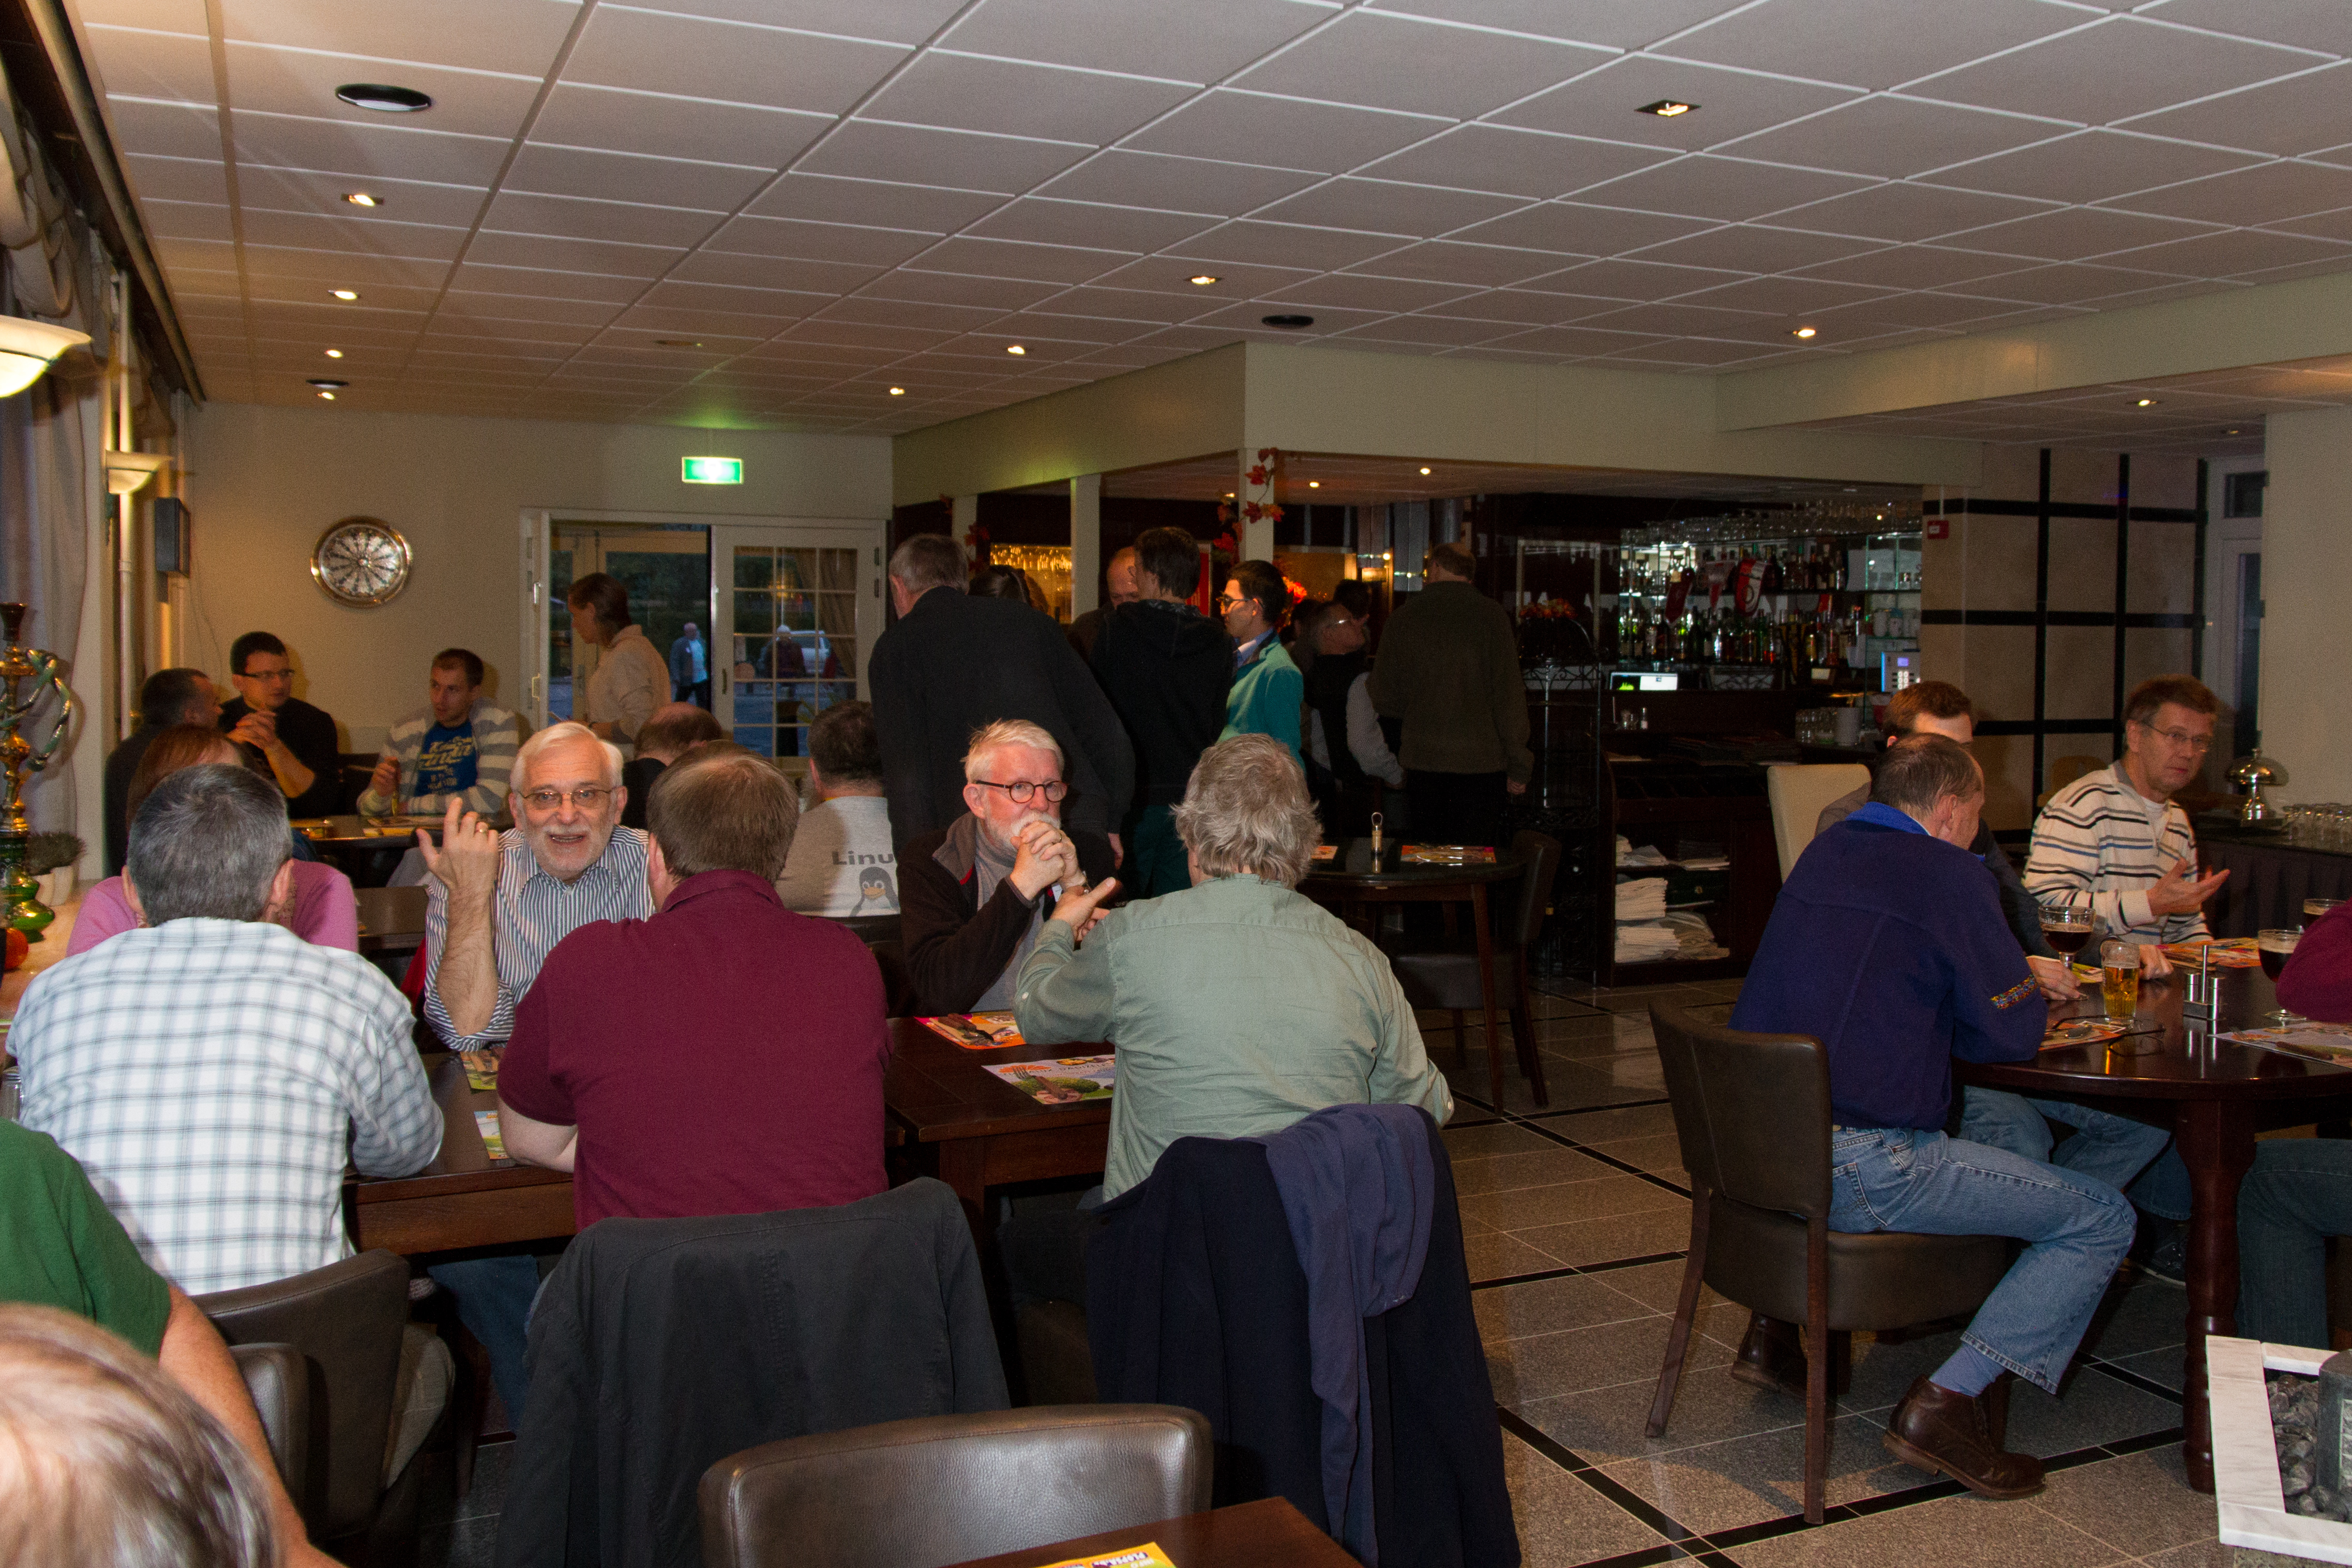
\includegraphics[width=0.85\textwidth]{IMG_2578}
\caption{Frühstück im \enquote{Scaldis} Hotel}
\end{figure}

Mit knapp 5000 Einwohnern ist Breskens zwar nicht der Nabel der Welt, der Ort liegt aber sehr schön an
 der Nordsee und bot genug Möglichkeiten, Nordsee-Flair aufzunehmen. Die vergleichsweise geringe
 Größe hatte auch den Vorteil, dass man jeden konferenz-relevanten Ort bequem zu Fuß erreichen
 konnte.

\section{Maandag}

Nach dem Frühstück im Hotel ging es dann am Montagmorgen in das \enquote{de Platte Knoop}, ein
 Café ganz in der Nähe des Deichs. Dort warteten ein offenes WLAN -- das mit der Zahl der Nutzer so
 seine Probleme hatte -- und Kaffee auf die Teilnehmer. Eine kurze Verzögerung gab es, als innerhalb von
 fünf Minuten nach dem allgemeinen Laptop-Anstöpseln die Sicherungen aufgaben: die
 Mehrfachsteckdosen waren wohl doch etwas einseitig verteilt gewesen!

\begin{figure}
\centering
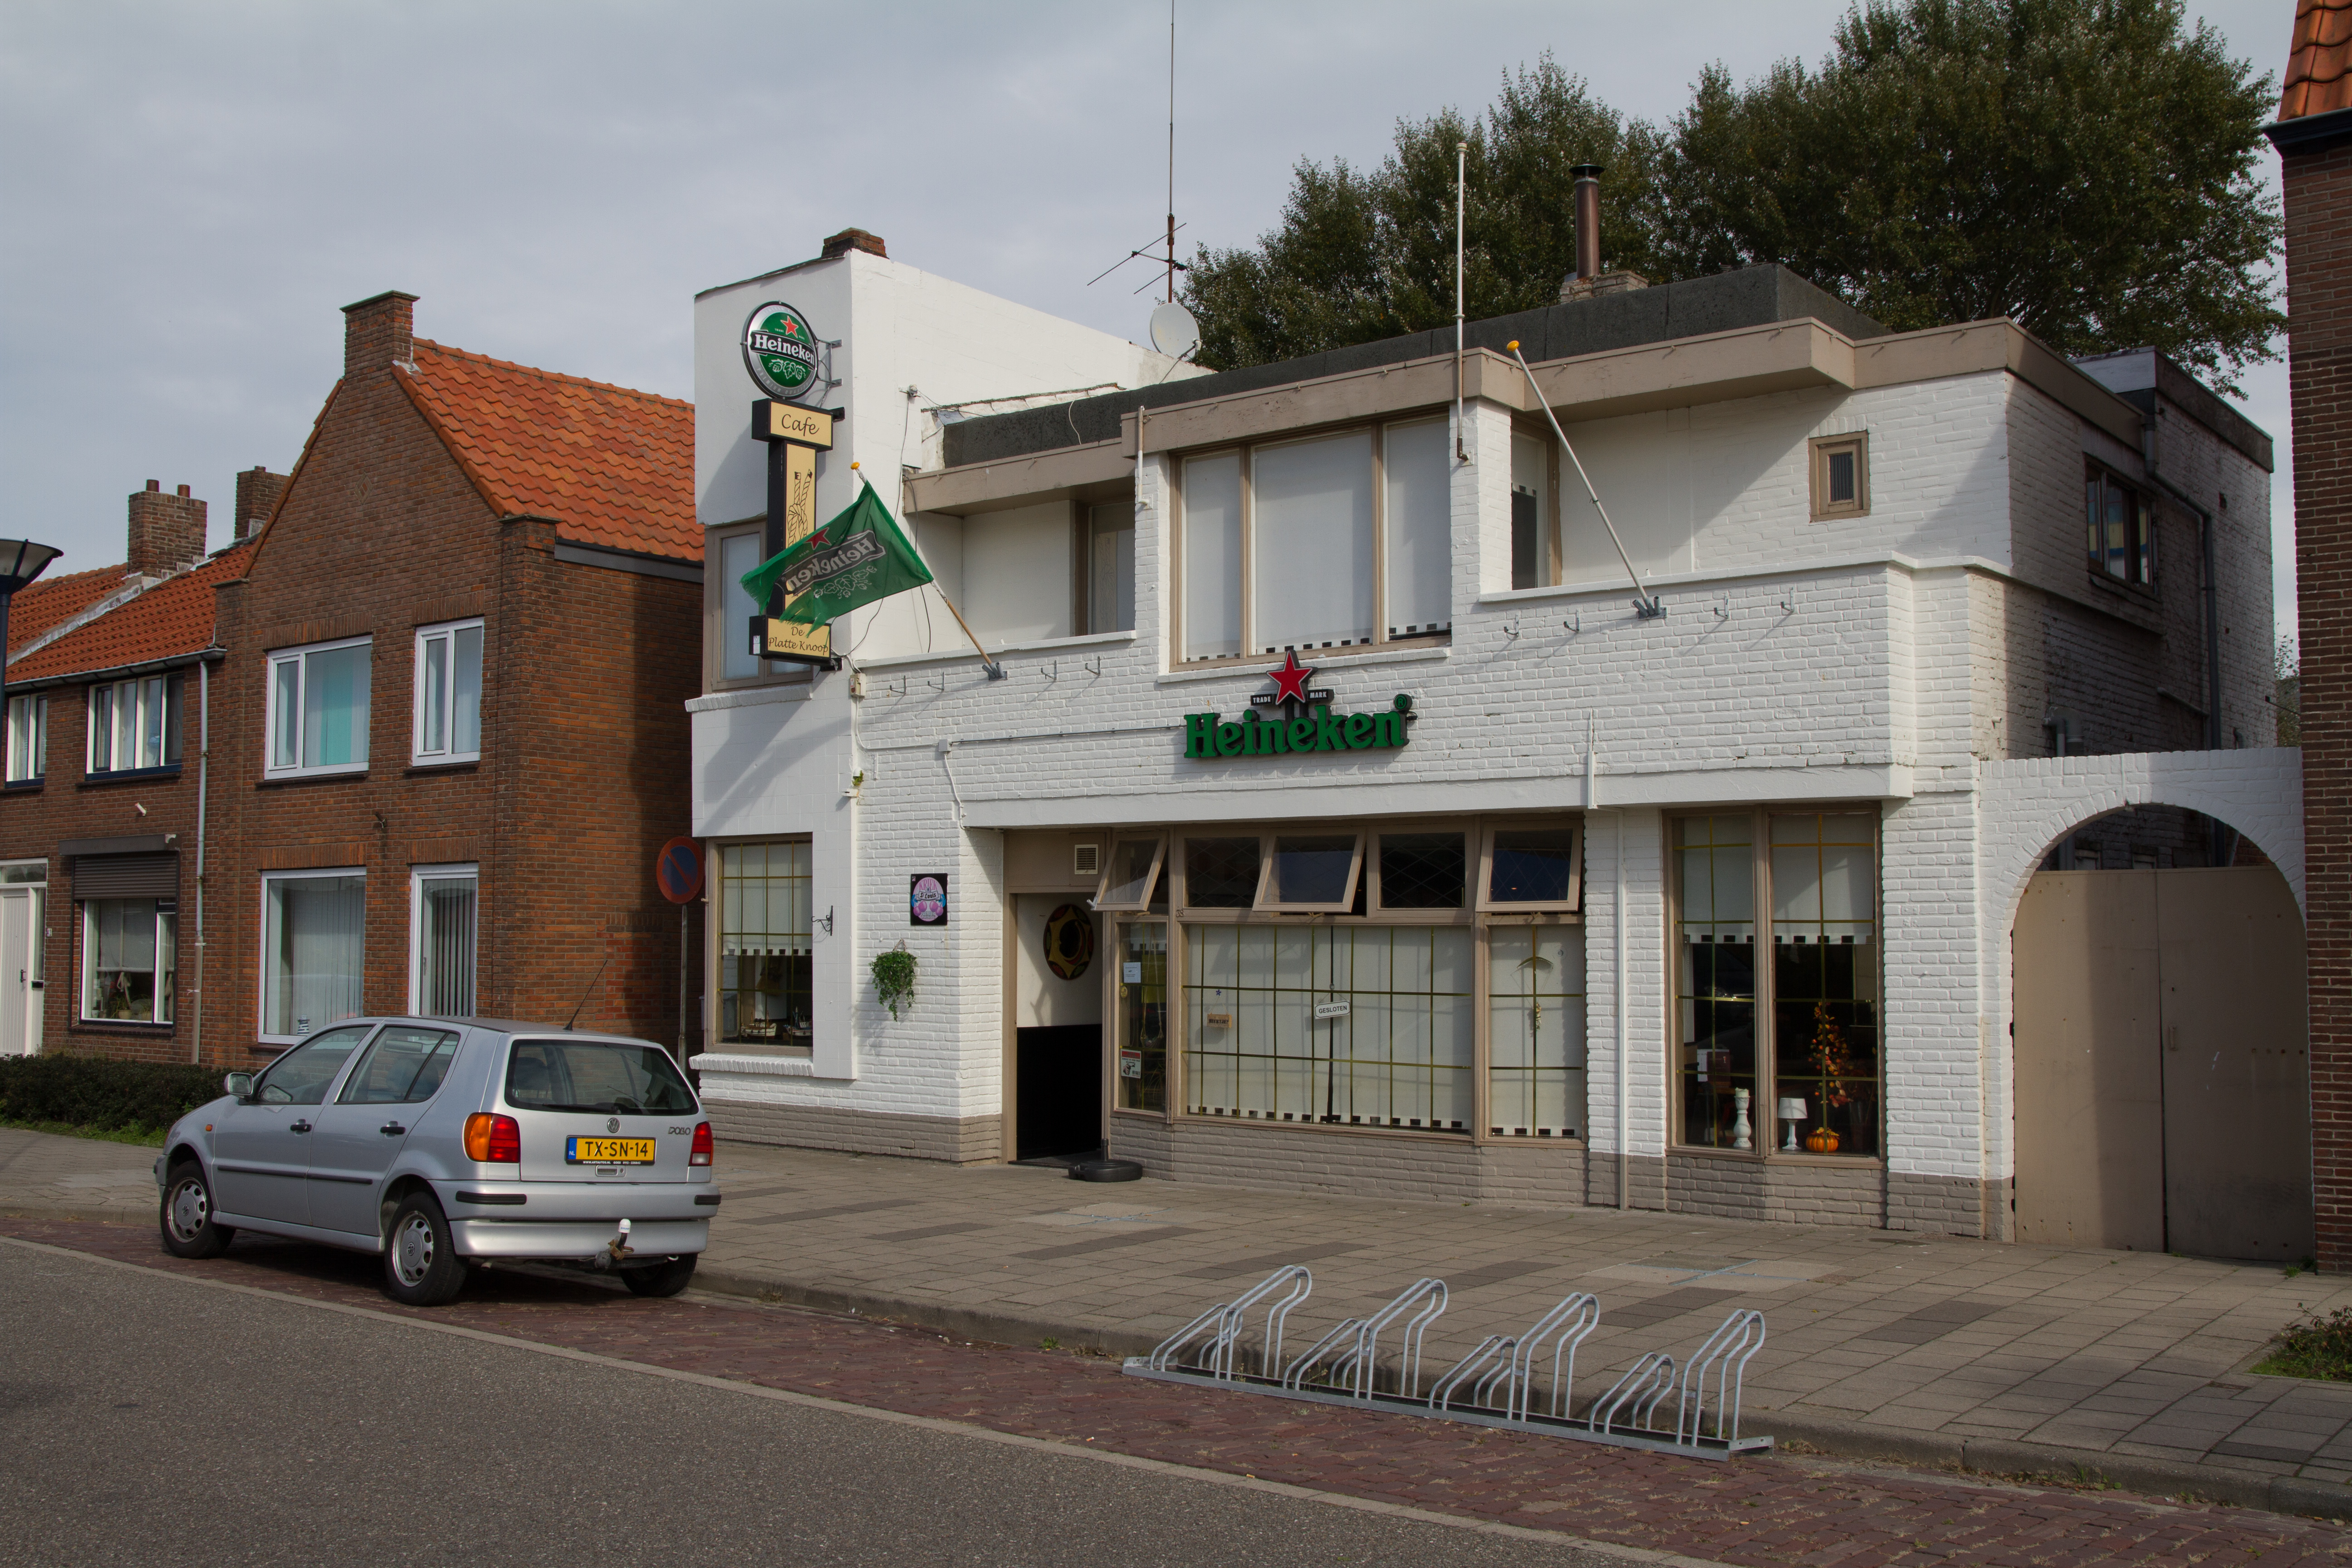
\includegraphics[width=0.85\textwidth]{IMG_2503}
\caption{Der Tagungsort \enquote{de Platte Knoop}}
\end{figure}

Die Schar der fast 50 Teilnehmerinnen und Teilnehmer war ähnlich bunt gemischt wie die Marken der
 zahlreich vorhandenen Laptops: neben der größten Gruppe aus Deutschland -- die Tagung war ja auch
 gleichzeitig die Dante Herbsttagung -- waren viele weitere Nationen vertreten. Aus Frankreich, Italien,
 Finnland, Polen, Tschechien, Norwegen und weiteren Ländern hatten \TeX ies den Weg nach Breskens
 gefunden. Die bei weitem weiteste Anreise hatten jedoch die drei japanischen Teilnehmer auf sich
 genommen!

Der erste Vortrag von Kees van der Laan zum Thema \enquote{Recreational \TeX\ \& Co - with a serious
 undertone} führte vor, dass man für verschiedenste Grafiken kein \LaTeX\ benötigt, da man ja Grafiken
 direkt in PostScript programmieren kann. Sehr interessant, ich werde aber wohl weiterhin auf PGF/TikZ,
 Inkscape und CorelDraw setzen. In einem weiteren Vortrag am Nachmittag zeigte Kees uns noch, wie
 man fraktale Julia-Mengen in PostScript darstellen kann.

Im Anschluss an Kees zeigte uns Jano Kula aus Tschechien, wie er für den Nike Run in Prag
 personalisierte T-Shirts in Con\TeX t erstellte.

Die textile Seite von \LaTeX\ \& Co war auch bei Mari Voipios Vorträgen das Thema. Sie erstellte
 Flechtmuster mit Metapost  und zeigte auch bei einem Workshop, wie man theoretisch und praktisch
 \LaTeX\ und Flechtarbeiten verbinden kann.

Nach einem Vortrag von Taco Hoekwater zum Thema Metapost hielt dann Patrick Gundlach zwei
 Vorträge. Im ersten Vortrag zeigte er die aktuelle Version seines \enquote{speedata} Publishing-Tools,
 das anhand von Regeln große Mengen Text auf Papier respektive eine PDF Datei bringen kann. 
Im zweiten Vortrag führte er vor, wie mittels Lua\TeX\ Callbacks Abstände in Dokumenten visuell
 dargestellt werden können, etwas, das mit Plain\TeX\ nur schwerlich -- falls überhaupt -- umsetzbar sein
 dürfte.

Nach den Vorträgen kamen wir dann mit der Dante Mitgliederversammlung zum offiziellen Teil des
 Abends, siehe dazu den entsprechenden Artikel in dieser DTK Ausgabe.

\section{Dinsdag}

Der Dienstag begann mit meinem eigenen Vortrag zum Thema \enquote{Reporting mit \LaTeX}, ein
 Artikel für die DTK folgt. Nach mir präsentierte Leo Arnold von der Technischen Universität München, 
wie man mit einem einzigen \LaTeX\ Lauf mehrere PDF Dateien erzeugen kann. Die von ihm selbst
 entwickelte Klasse erzeugt auf der Basis von \texttt{comment.sty} und \texttt{write18} weitere
 Instanzen von \texttt{pdflatex}, die dann die einzelnen Versionen ausgeben. Ich hatte bisher
 angenommen, dass dies nicht möglich sei und freue mich, wenn diese Technologie in Klassen- oder
 Paketform auf CTAN kommt.

Vor der Mittagspause präsentierte Taco Hoekwater, der lokale Organisator der Konferenz, noch zu den
 Themen \enquote{Pfadauflösung in Metapost} und \enquote{Parsen von PDF Content Streams}.

Den Nachmittag nutzte Hans Hagen dann, um verschiedene Con\TeX t Themen vorzustellen, gefolgt von
 Luigi Scarso, der zu \enquote{MFLua} präsentierte.

Zum Abschluss des Abends hatte man Gelegenheit, mit Willi Egger Konferenzmappen zu basteln.

\section{Woensdag}

\begin{figure}
\centering
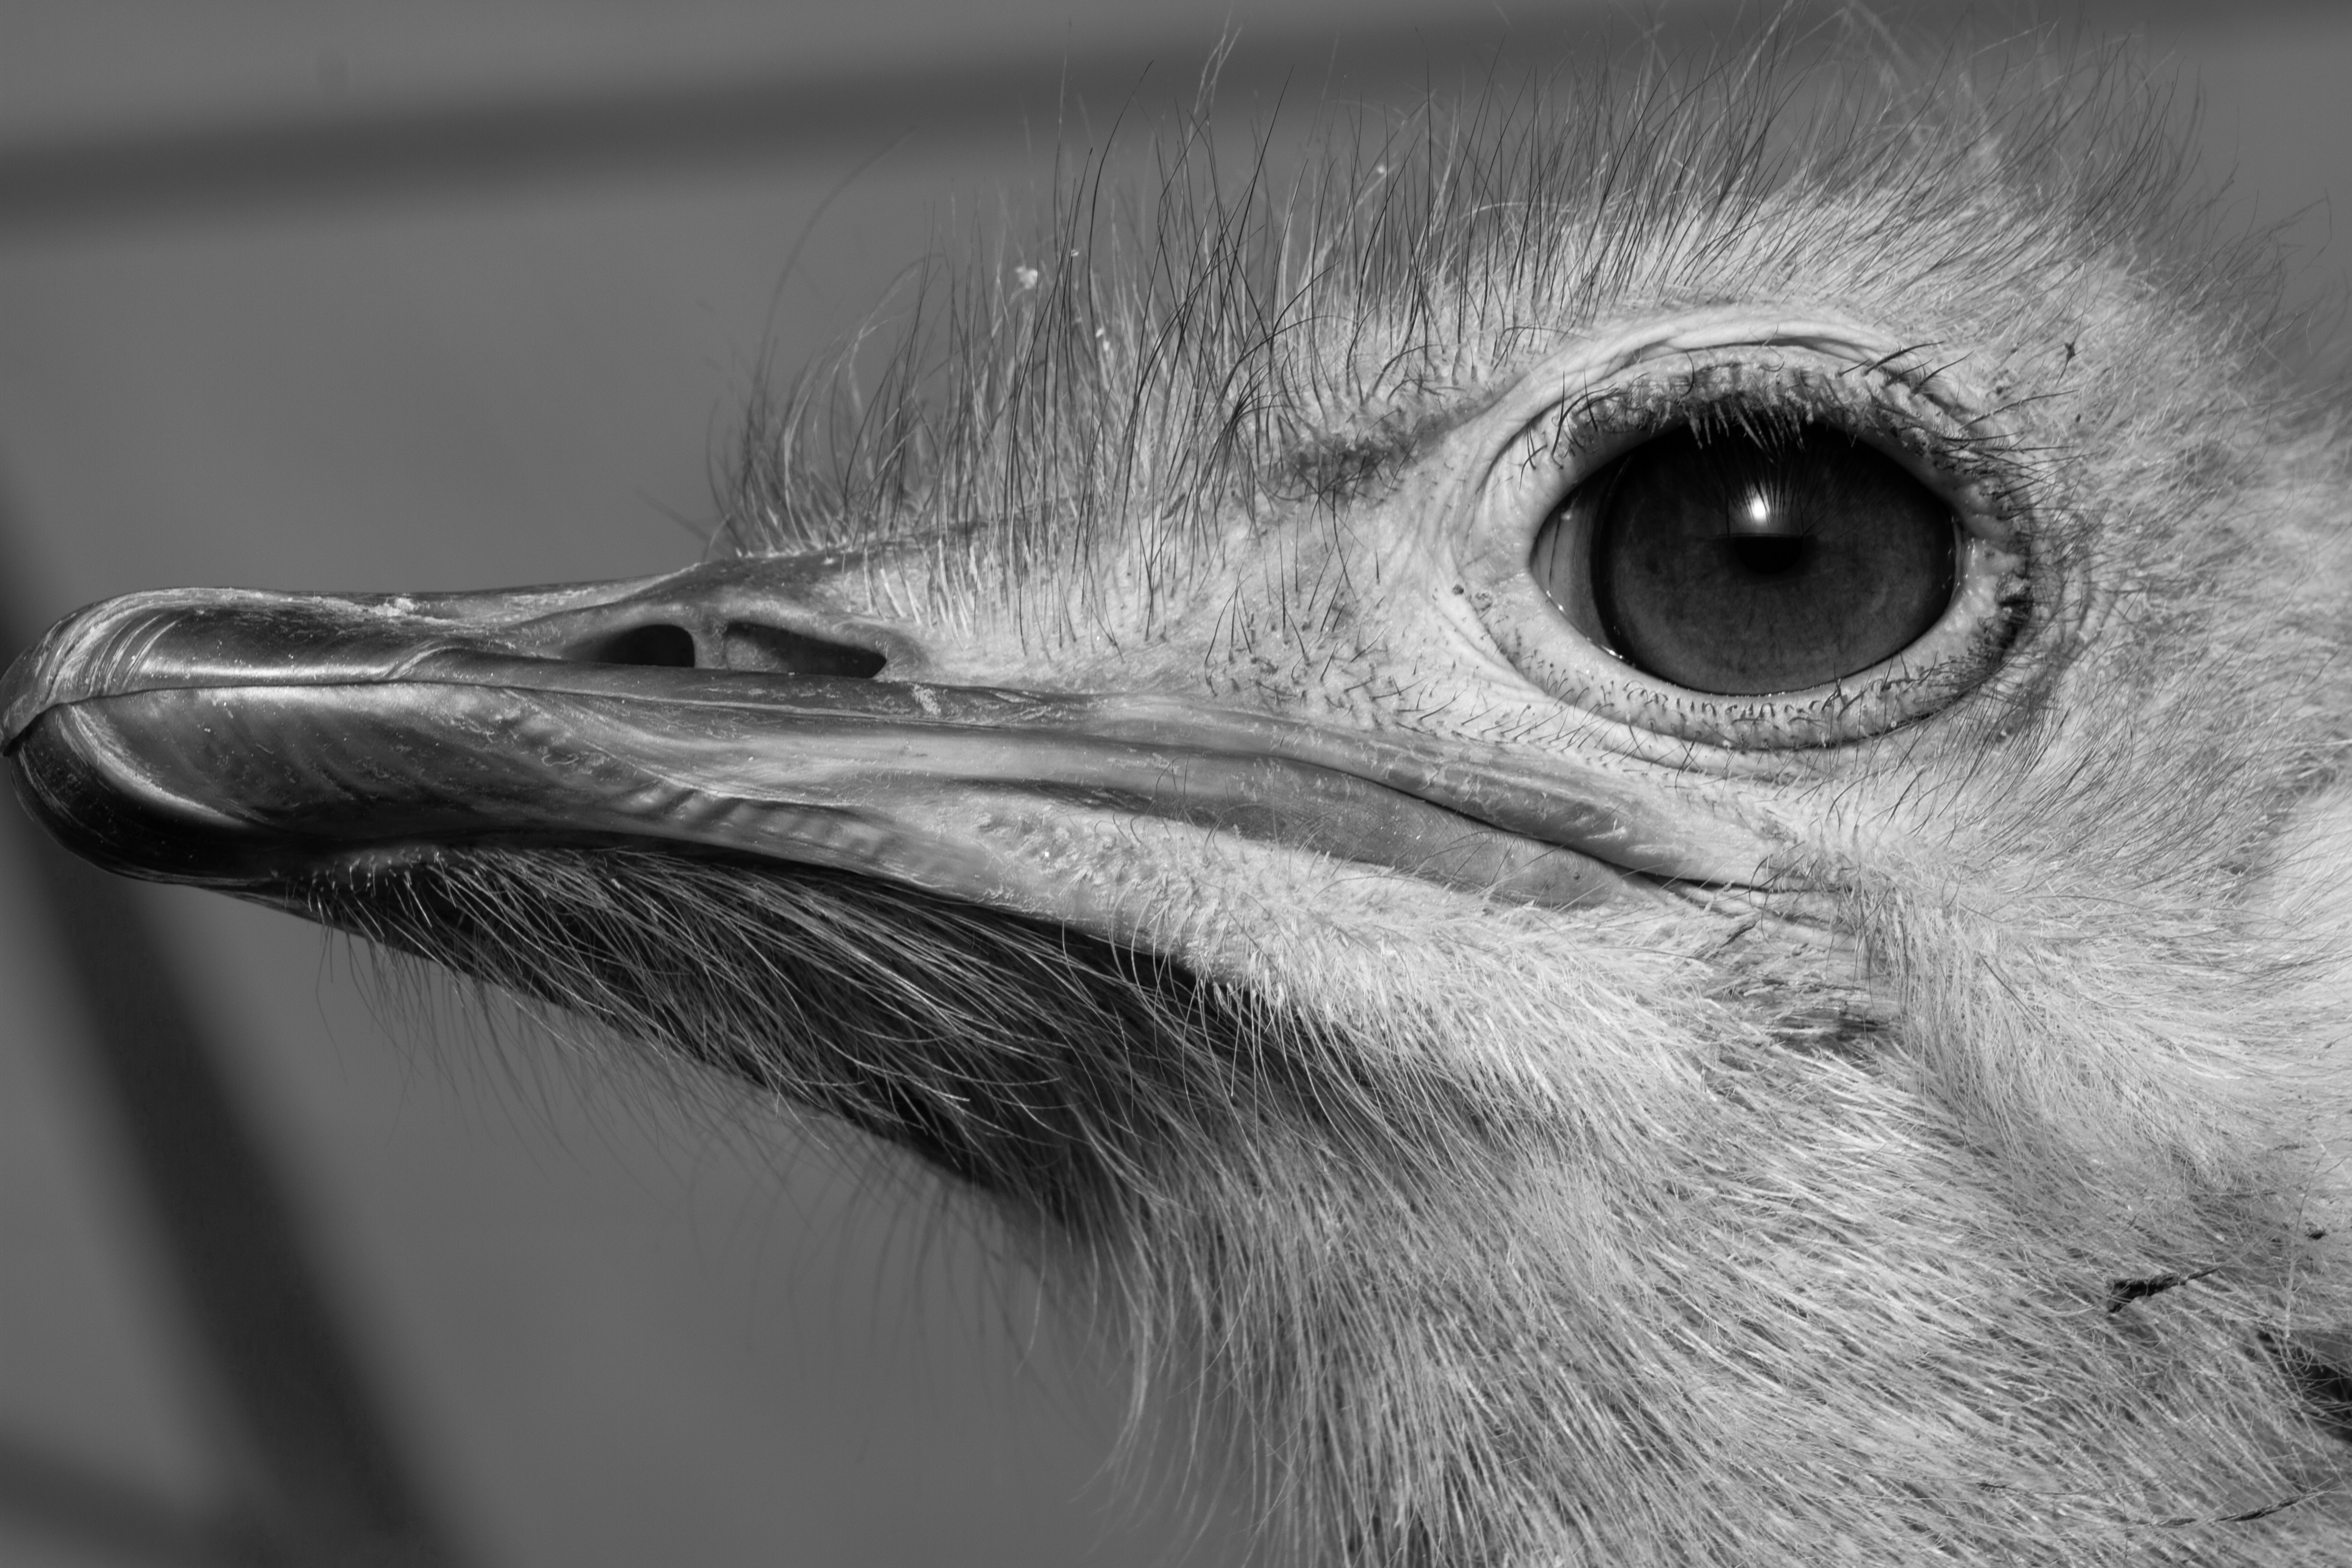
\includegraphics[width=0.85\textwidth]{IMG_2950}
\caption{Auf der Straußenfarm}
\end{figure}


Der Mittwoch stand ganz im Zeichen des touristischen Beiprogramms. Morgens um 9 Uhr stand ein
 original amerikanischer Schulbus abfahrbereit, der erste Stop war dann auf einer Straußenfarm, wo wir
 mit Kaffee und Kuchen\footnote{aus Straußeneiern, ein Ei reicht dabei für sieben (!) Kuchen} begrüßt
 wurden. Die Fotoapparate standen bei den meisten dann auf Dauerfeuer, als wir uns die kleinen und großen Strauße anschauten.

\begin{figure}
\centering
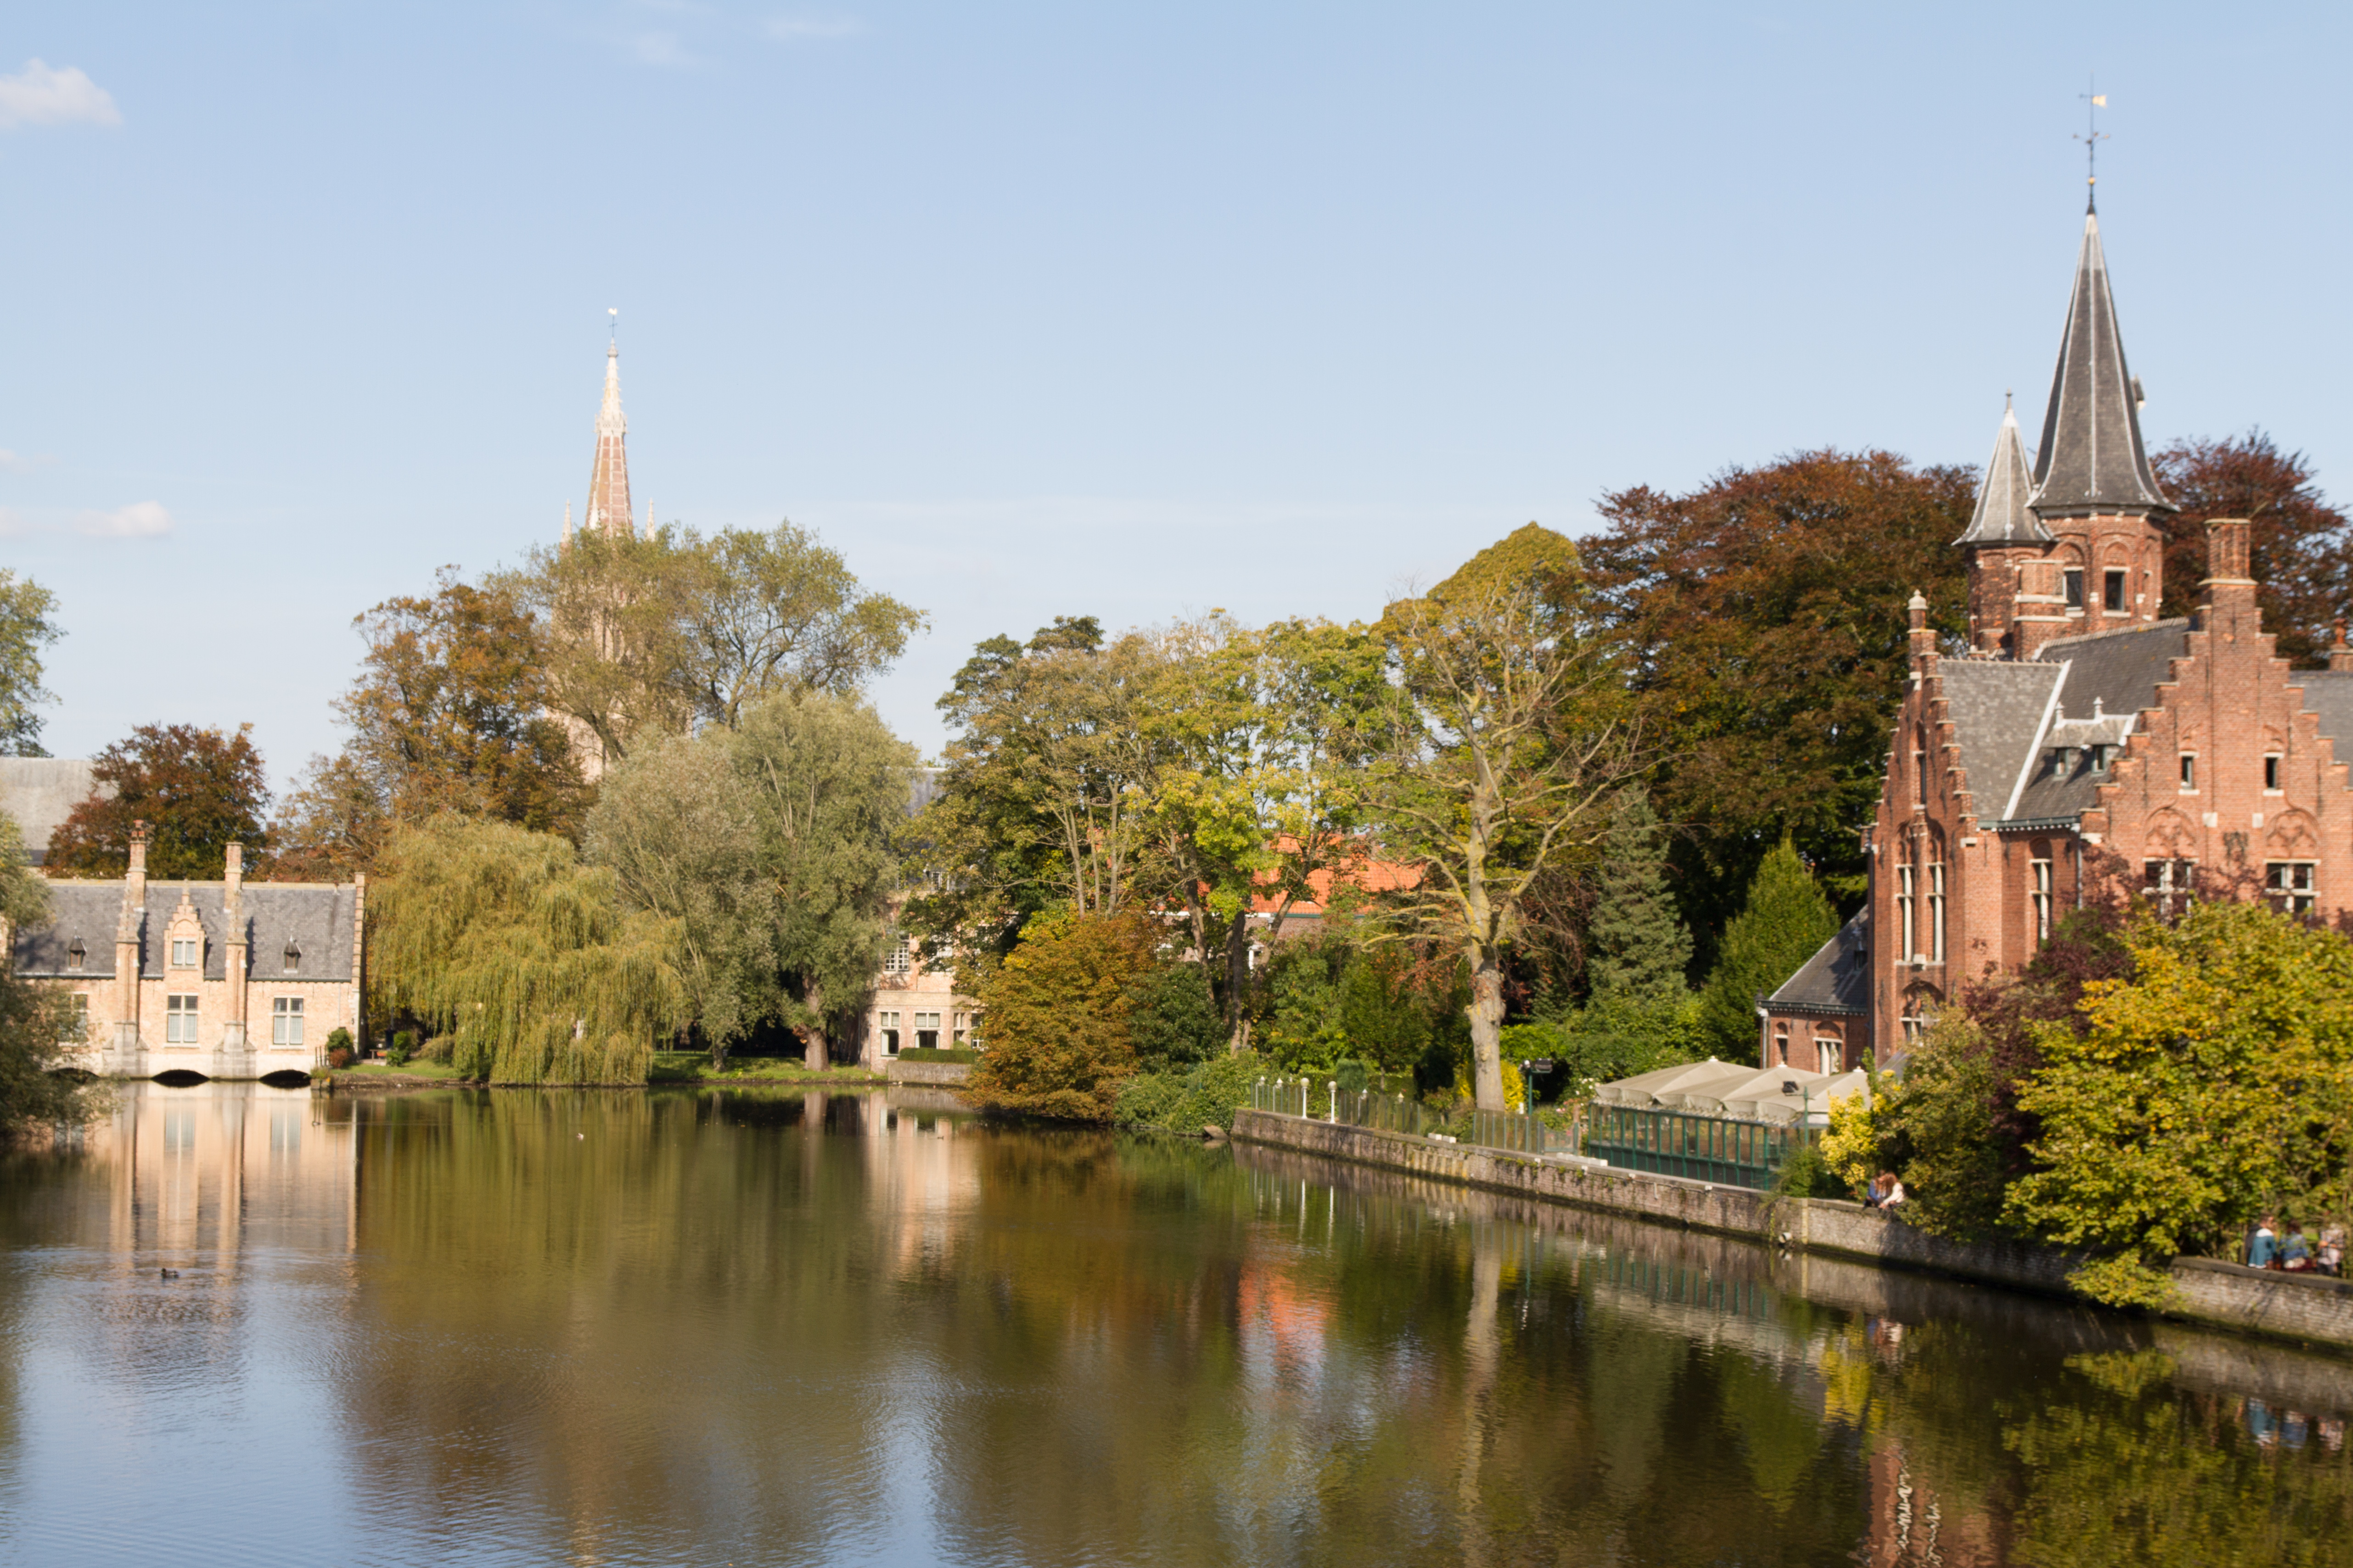
\includegraphics[width=0.85\textwidth]{IMG_3210}
\caption{Brügge, am \enquote{Minnewater}}
\end{figure}


Nach dem Mittagessen in einem Landgasthof (der über ein offenes WLAN verfügte) ging die Reise nach Brügge. Brügge, seit dem 2.~Jahrhundert besiedelt, war aufgrund von Hanse-Mitgliedschaft und günstiger geografischer Lage einst die reichste Stadt  Nordeuropas. Dieser Reichtum ist auch heute noch sichtbar, davon konnten wir uns bei der Stadtführung überzeugen. Die verbleibende Zeit bis zur Abfahrt des Busses nutzten dann alle, um sich noch einige Sehenswürdigkeiten anzuschauen oder in den unzähligen Schokoladengeschäften Brügges exzessiv zu shoppen (zumindest ging es mir so).

\begin{figure}
\centering
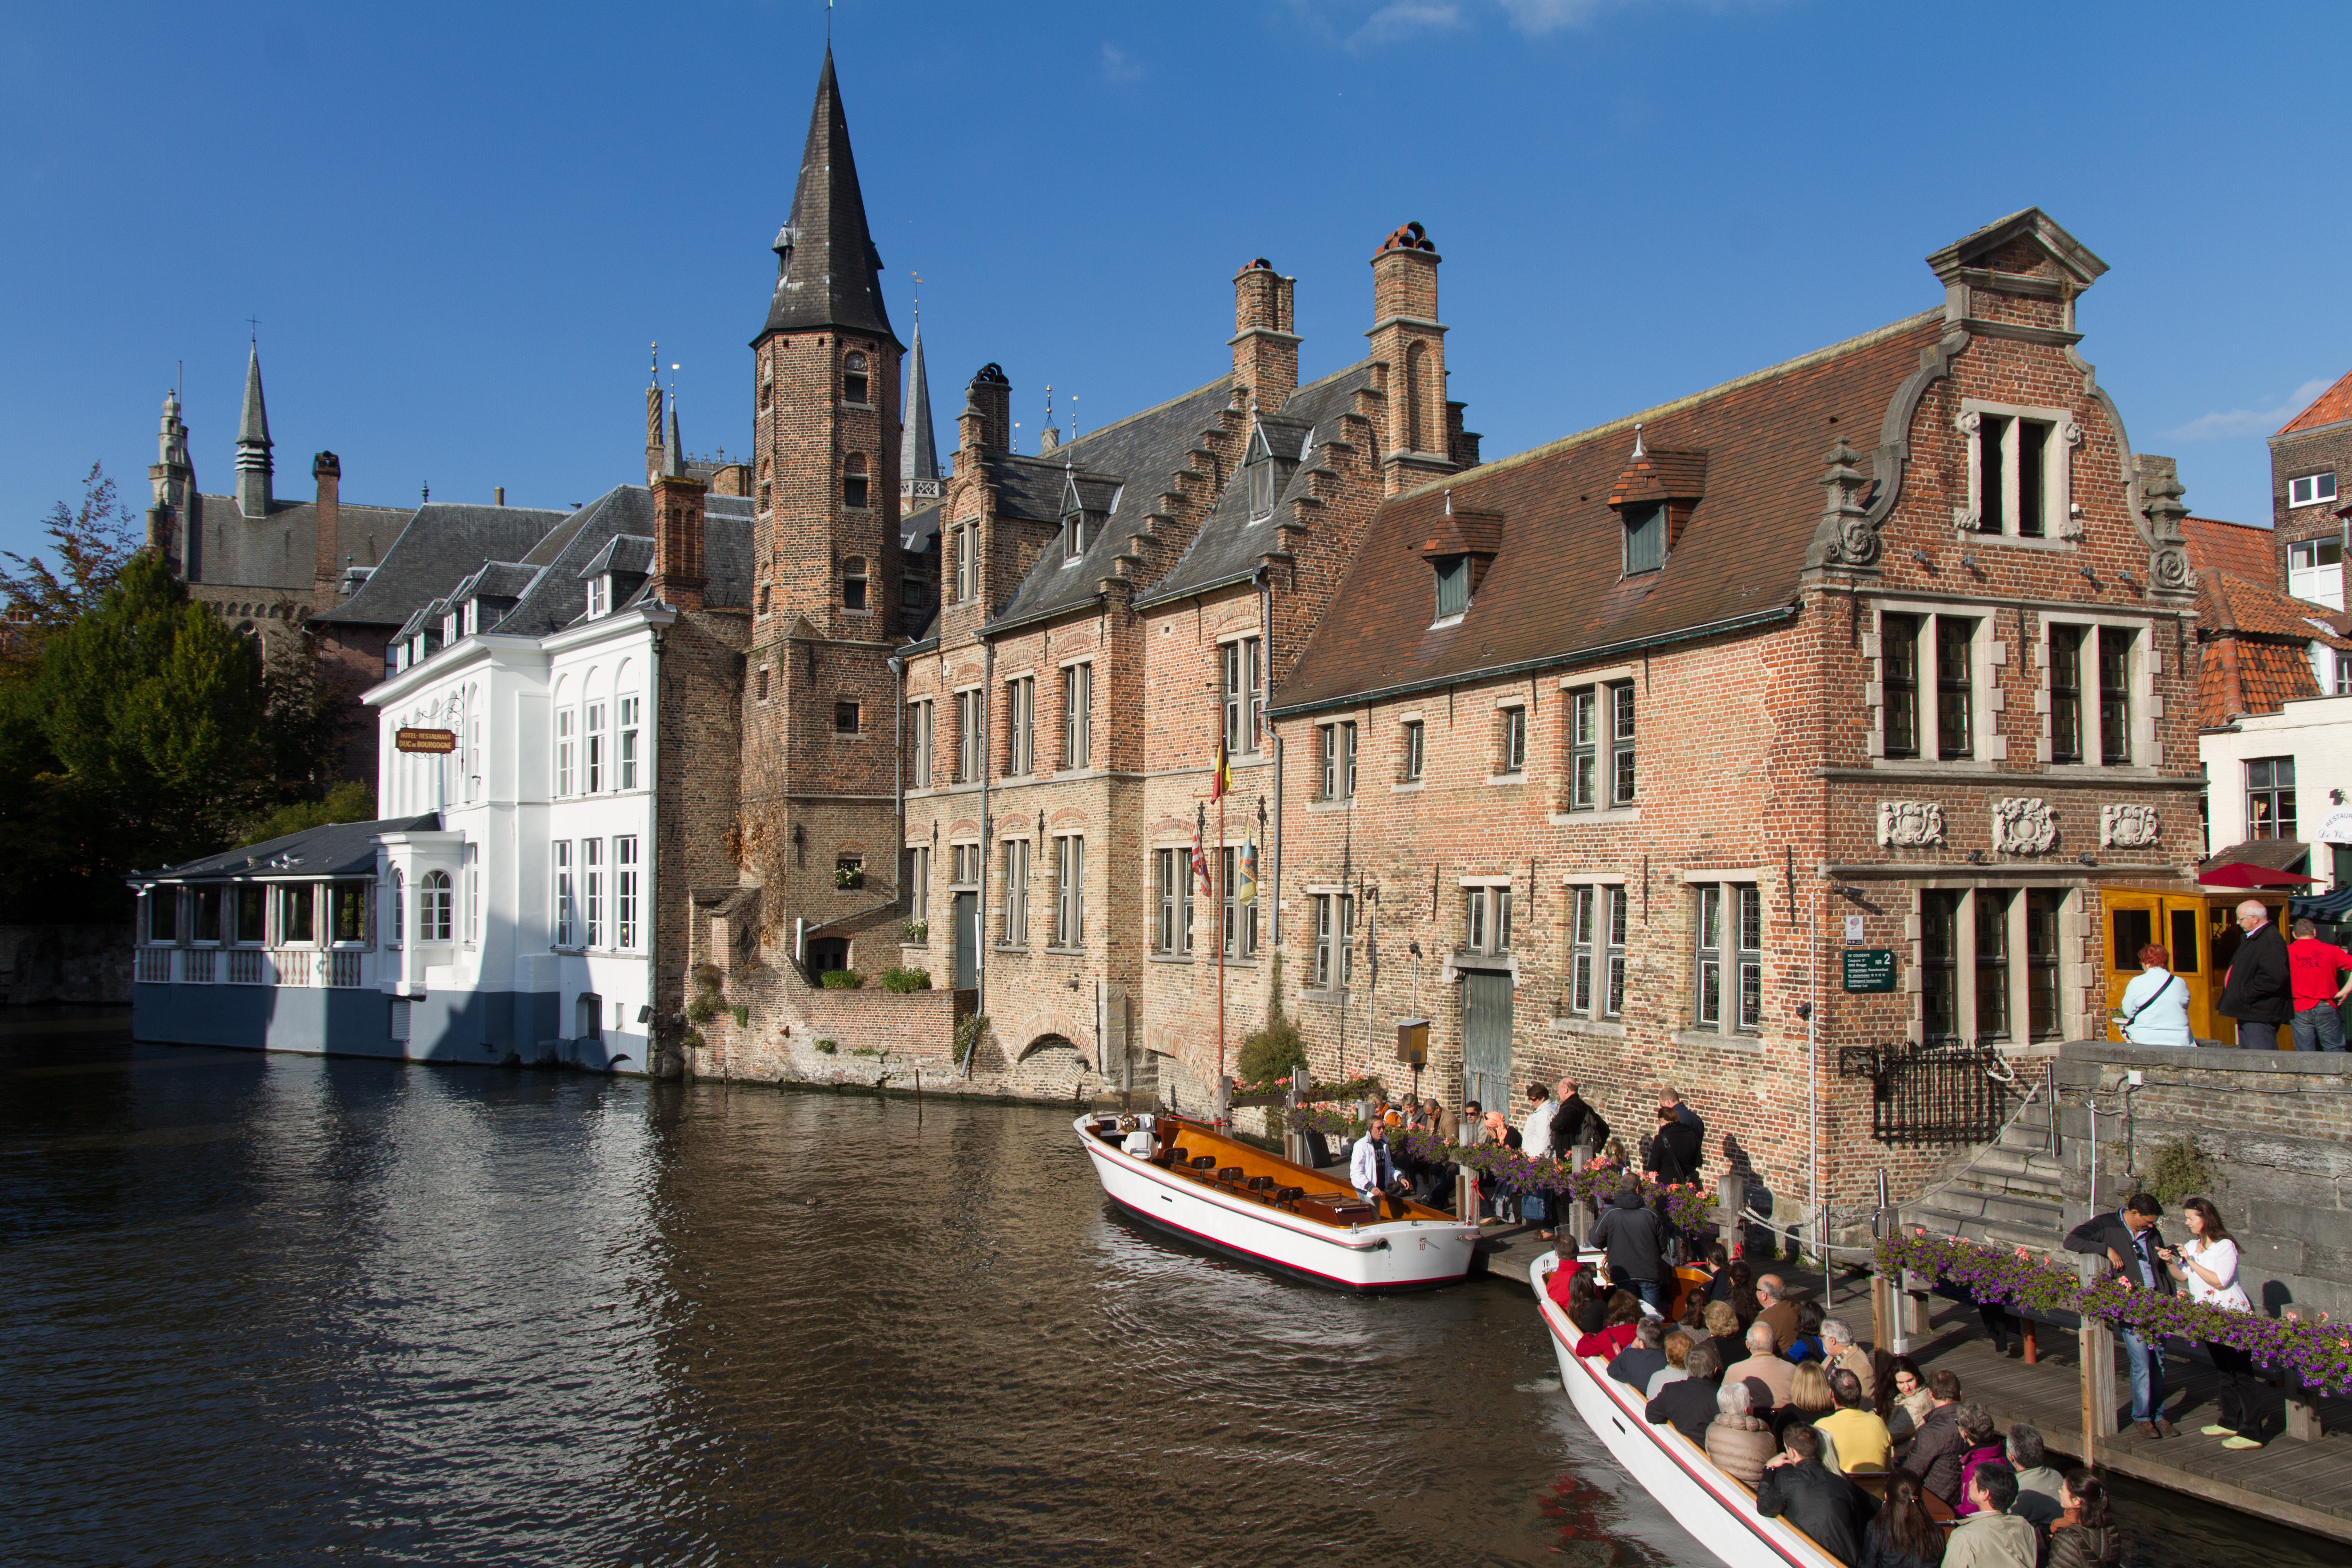
\includegraphics[width=0.85\textwidth]{IMG_3350}
\caption{Brügge, am \enquote{Dijver}}
\end{figure}

Bevor es dann zum Konferenzdinner in ein sehr gutes Breskener Restaurant ging, kehrten wir noch in einem Spirituosenladen ein, wo es niederländischen Gin, sogenannten \enquote{Geneva}, mit Austern gab.

\section{Donderdag}

Der Donnerstag begann mit mehreren Vorträgen zu Fonts. Bogus\l av Jackowskim, Jerzy Ludwichowski und Piotr Strzelczyk von der GUST zeigten die Abläufe zur Erstellung der mathematischen \TeX Gyre Fonts, präsentierten den aktuellen Stand des Projekts und sprachen über die Abwärtskompatibilität von LM Math und CM Math.

Nach dem Mittagessen erfüllte Hans dann einen Wunsch von mir und zeigte den Anwesenden die absoluten Con\TeX t Grundlagen. Da das aktuelle Con\TeX t auf Lua-Basis arbeitet, besteht kein Grund mehr, Ruby etc. installiert zu haben, ein aktuelles \TeX\ Live reicht aus. Nach diesen Grundlagen ging es dann ans Eingemachte, als Hans über das Rechnen in Tabellen mit Lua, das Parsen von XML-Dateien und die Anbindung an MySQL Datenbanken sprach.

Beendet wurde der Tag mit einem Besuch beim Glasbläser, der aus glühend heißem Glas Schalen und Glastiere formte.

\section{Vrijdag}

Am Freitag hatten die Teilnehmer mit der weitesten Anreise, Munehiro und  Hironori aus Japan, das Wort. Sie sprachen über die Nutzung von \LaTeX\ in japanischen Satzhäusern und die Schwierigkeiten, die der japanische Satz mit seiner Vielzahl von Zeichen und unterschiedlichen Satzrichtung hat. Über diese Präsentation hat sich auch ein japanischer Freund von mir gefreut, dem ich die PDF-Datei noch während der Präsentation zukommen ließ und der darin einige seiner \LaTeX-Probleme behandelt sah.

Wer mehr zum japanischen Textsatz mit \LaTeX\ erfahren möchte, der kann dies übrigens im nächsten Jahr in Tokyo tun, wo Ende Oktober 2013 die TUG Konferenz stattfinden wird.

Neben Hans, der noch mehr über Con\TeX t berichtete, sprachen am Freitag noch Ivo Geradts und Kai Eigner über den Satz von Sanskrit mit Lua\TeX\, Tomás Hála über Unterschiede im Satz von Tschechisch und Slovakisch, bevor Jean-Michel Hufflen über die Fortschritte bei der Entwicklung seines MIBib\TeX\ referierte. 

Beschlossen wurde die Euro\TeX\ 2012 dann von Sietse Brouwer, der mit den Anwesenden über mögliche Verbesserungen an der Con\TeX tgarden Webseite sprach.

\section{Odyssee -- Rückfahrt mit Hindernissen}

Die Rückfahrt nach Köln mit Doris und Ulrik war auch mit Spannung und Dramatik gespickt. Den ersten unfreiwilligen Stop hatten wir in Hoofdplaat, nur wenige Autominuten von Breskens entfernt, als sich Doris' Opel Kadett und ein niederländischer Toyota Yaris auf der Kreuzung ein wenig zu nah kamen. Es gab glücklicherweise nur geringen Blechschaden, daher konnten wir die Fahrt nach kurzer Zeit fortsetzen. 

Eine weitere unfreiwillige Unterbrechung gab es dann nur noch in Belgien, als nach kurzer Rast im Heim  von Ronald McDonald das Auto nicht mehr anspringen wollte. Beherztes Anschieben bei eingelegtem Gang war dann angesagt, die restliche Reise lief dann -- zwar bei strömendem Regen -- problemlos.

\section{Fazit}

Was bleibt sind die Erinnerungen an eine tolle Tagung, die dank Tacos toller Organisation für alle Teilnehmer viel Spannendes und Lehrreiches bot. Auch wenn einige Themen jenseits von dem angesiedelt waren, was ich in \LaTeX\ kann, kenne  oder benötige, so bot diese Tagung viele Einblicke in das, was \TeX nisch möglich ist. 




\begin{figure}
\centering
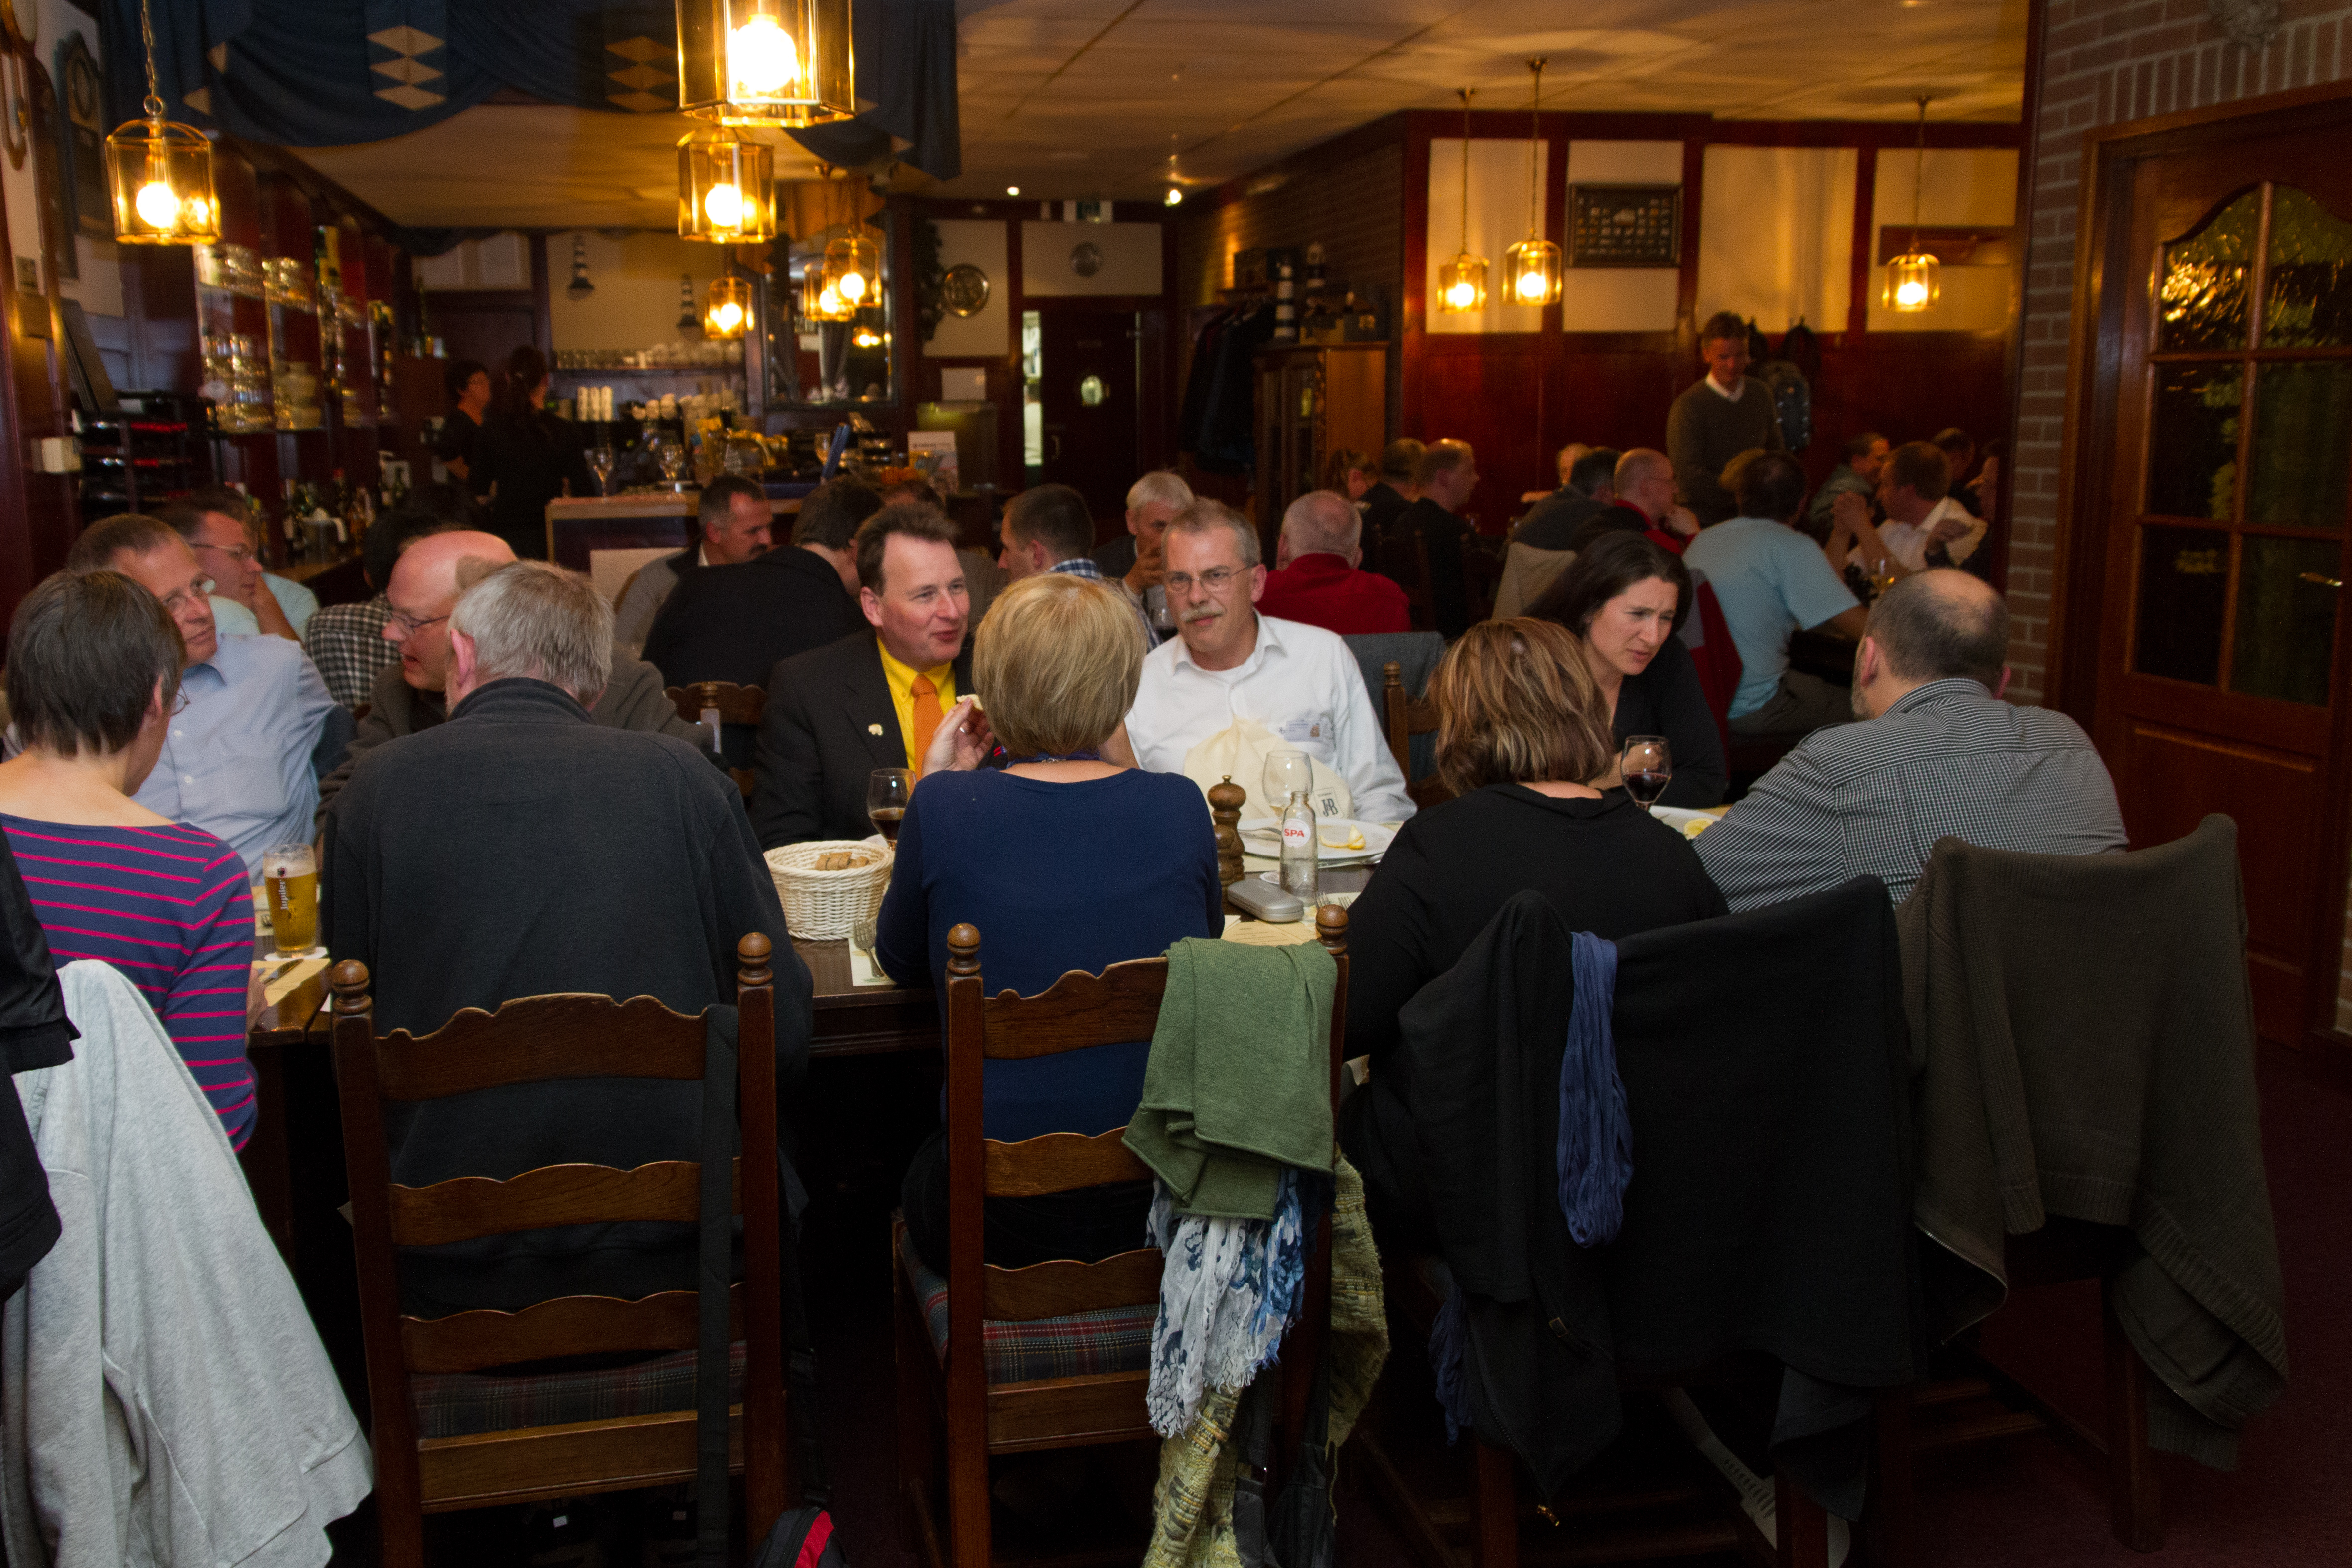
\includegraphics[width=0.85\textwidth]{IMG_3582}
\caption{Konferenzdinner in Breskens}
\end{figure}
\end{document}


